\documentclass[letterpaper]{article}
\usepackage{natbib,alifeconf}

\usepackage{subfig}


\usepackage{xcolor}

\usepackage{fancybox}
%Fancy List
\definecolor{solarized@base03}{HTML}{002B36}
\definecolor{solarized@base02}{HTML}{073642}
\definecolor{solarized@base01}{HTML}{586e75}
\definecolor{solarized@base00}{HTML}{657b83}
\definecolor{solarized@base0}{HTML}{839496}
\definecolor{solarized@base1}{HTML}{93a1a1}
\definecolor{solarized@base2}{HTML}{EEE8D5}
\definecolor{solarized@base3}{HTML}{FDF6E3}
\definecolor{solarized@yellow}{HTML}{B58900}
\definecolor{solarized@orange}{HTML}{CB4B16}
\definecolor{solarized@red}{HTML}{DC322F}
\definecolor{solarized@magenta}{HTML}{D33682}
\definecolor{solarized@violet}{HTML}{6C71C4}
\definecolor{solarized@blue}{HTML}{268BD2}
\definecolor{solarized@cyan}{HTML}{2AA198}
\definecolor{solarized@green}{HTML}{859900}
\definecolor{solarized@darkgreen}{HTML}{006400}

\usepackage{listings}

\lstset{
    language=python,
    columns=fixed,
    tabsize=2,
    extendedchars=true,
    breaklines=true,
    frame=single,
    numbers=left,
	numberstyle=\tiny,
    numbersep=5pt,
    rulesepcolor=\color{solarized@base03},
    numberstyle=\tiny\color{solarized@base1},
    basicstyle=\footnotesize\ttfamily,
    keywordstyle=\color{magenta},
    stringstyle=\color{solarized@base00}\ttfamily,
    identifierstyle=\color{solarized@blue},
    commentstyle=\color{solarized@base1},
    emphstyle=\color{solarized@red},
    backgroundcolor=\color{solarized@base3},
    literate={ö}{{\"o}}1
    {ä}{{\"a}}1
    {ü}{{\"u}}1
    {Ö}{{\"O}}1
    {Ä}{{\"A}}1
    {Ü}{{\"U}}1
}
\lstset{
 morekeywords={OPTIONS, TITLE, LET, PROC, SURVEYSELECT, NOPRINT, SORT, MEANS, DATA, MEND, MACRO, RUN, SQL, QUIT, UNIVARIATE, SURVEYMEANS, SELECT, INTO, FROM, PUT,BY,SET,VAR,OUTPUT,SAMPRATE,REP,SEED, STRATA,ALLOC,END,IF,THEN,ELSE,MERGE,KEEP,RENAME,DO,HISTOGRAM,OUT,METHOD,STATS,RATE,WEIGHT,STATISTICS,ODS, MEAN,SUM},
 moredelim=[is][\color{solarized@darkgreen}]{|}{|}
 morecomment={total}
}


\pagenumbering{roman}


\title{Bootstrapping the Support Vector Machine}

\author{Thomas Goerttler$^{1,2,3}$, Christian Koopmann$^{1,2,3}$, Patricia Craja$^{1,2,3}$ \\
\mbox{}\\
$^1$Humboldt University of Berlin, Unter den Linden 6, 10099 Berlin \\
$^2$Free University Berlin, Kaiserswerther Str. 16-18, 14195 Berlin \\
$^3$Technische Universität Berlin, 10623 Berlin \\
thomas.goerttler@gmail.com\\
c.k.e.koopmann@gmail.com\\
Patricia.craja@gmx.de\\
}


\begin{document}
\maketitle

\begin{abstract}
	Support Vector Machines are one of the most successful methods of Machine Learning. After training they can predict for each point a possible class. Unfortunetly there is not uncertaincy captured, that the point is really in this class. We found out a way to calculate variance for a support vector machine. We use bootstrapped samples and take this into account. The variance can be calculated parallized.
\end{abstract}

\section{Introduction}

Support Vector Machines are one of the most successful methods of Machine Learning. By reducing non-linear complex decisions problems to linear problems through application of the kernel-Trick, they represent a computationally efficient way to tackle these problems. 

svm uses hyperlance space feature to seperate data. The dimension of feature space ist controlled by choice of kernel function. Commen Kernels are the linear kernel, the gausian kernel (rbf) and the polynomial kernel.

SVMs based on certain kernels (e.g. Gaussian RBF Kernel) are non parametric methods. Since the distribution of the underlying data is generally unknown so is the finite sample distribution of these methods. 
There has been considerable research on the asymptotic distribution of SVMs, which have been shown to be asymptotically normally distributed under certain con- ditions. An alternative idea to estimate these distributions is using Efrons empirical boot- strap. The idea behind this method is to repeatedly draw samples with replacement from the full data according to the empirical distribution function of the data. Through the repeated calculation of the statistic of interest one can get an estimate of its distribution. For the SVM this estimate has been shown to be consistent under relatively mild conditions.
..
\section{Background}

What is the status in the science world right now.
Important has been \textbf{bootstrap, distances and parallelization}

\section{Problem}

There is noy way to calculate uncertaincy (variance) of the prediction as we have no assuptions about the distribution.We found out that we can sample variance by bootsrapping.
Futhermore we found out that they are tuning parameter, data-distribution option and svm attributes that influce this variance.

Predictions are only binary variables and therefore might be identical across all bootstrap samples Therefore we use minimal distance of predictionpoint to decision boundary as real valued substitue 



\begin{figure}[!htb]
\begin{center}
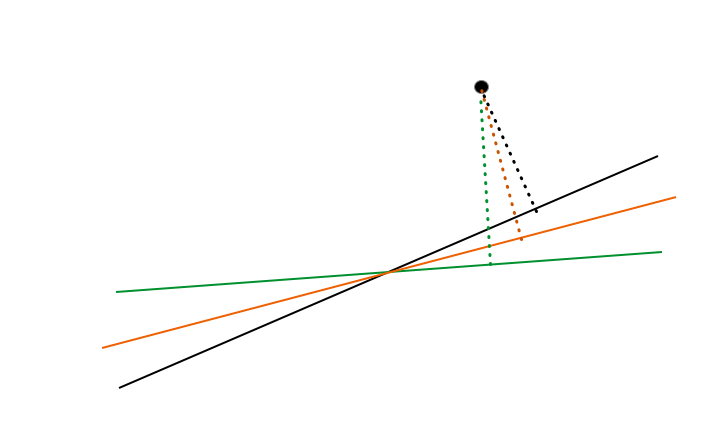
\includegraphics[width=1.5in]{abb/distances.jpg}
\caption{Really awesome trick of distance}
\label{fig1}
\end{center}
\end{figure}

\begin{figure}[!htb]
\begin{center}
\subfloat[]{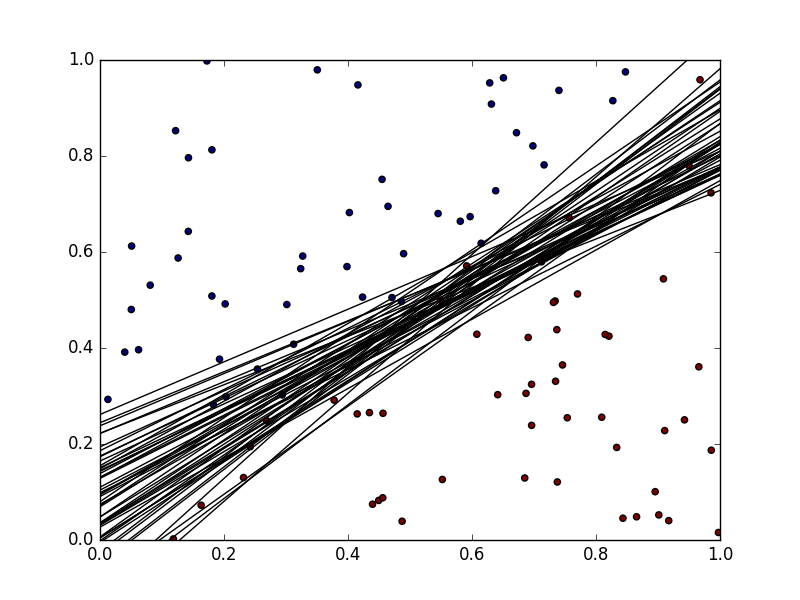
\includegraphics[width=1.5in]{abb/100_n.jpg}}
\subfloat[]{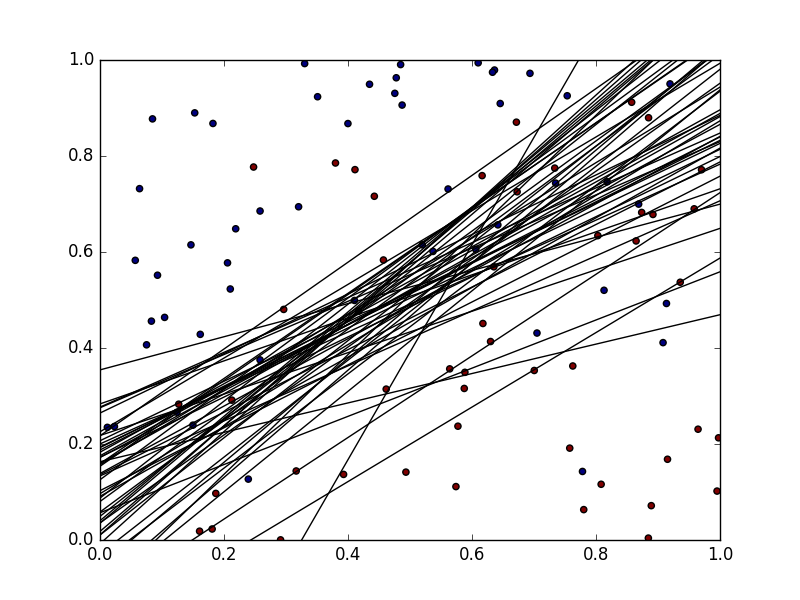
\includegraphics[width=1.5in]{abb/100_y.jpg}}

\subfloat[]{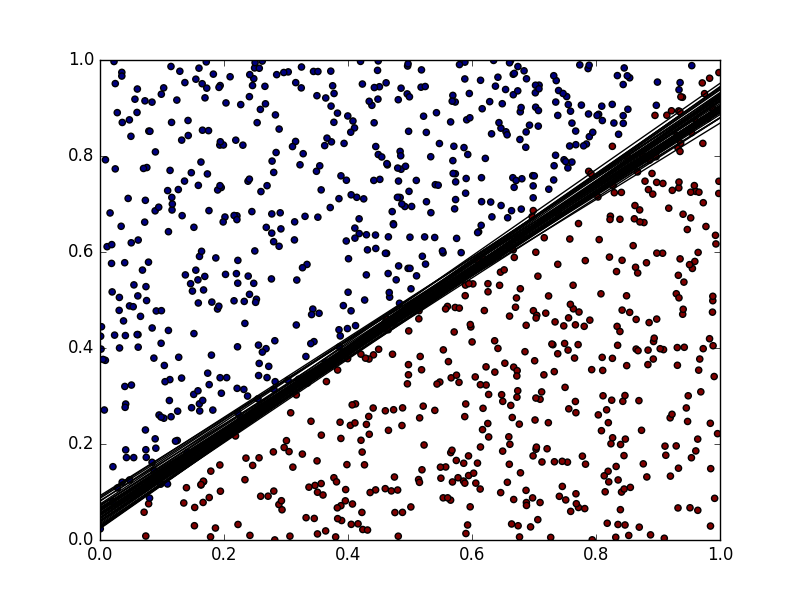
\includegraphics[width=1.5in]{abb/1000_n.jpg}}
\subfloat[]{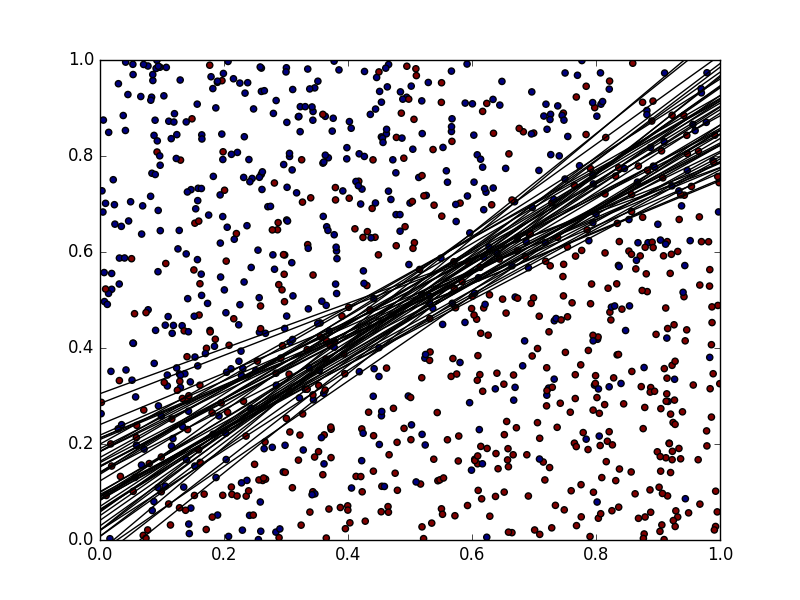
\includegraphics[width=1.5in]{abb/1000_y.jpg}}
\caption{(a) They are 100 perfectly seperated points, (b) They are 100 not perfectly seperated points ...... }
\label{fig1}
\end{center}
\end{figure}


\section{Implementation}



\begin{figure}[!htb]
\begin{center}
\begin{lstlisting}
def bootstrap_the_svm(trainings_data, prediction_data, kernel, C, gamma = "auto", degree = 3, processes = 10, replications = 1000):

    input_parameters = SVM_Input(trainings_data, prediction_data, kernel, C, gamma, degree)
    data = input_parameters
    real_svm = do_svm(data)
    
    ### Do bootstrapping
    PROCESSES = processes
    REPLICATIONS = replications
    pool = Pool(processes = PROCESSES)
    results = pool.map(single_sample_and_svm, [data] * REPLICATIONS)
        
    ### Calculate the Variance of the Support Vector Machine
    
    points_information = Points_Information(results)
    
    variance_of_svm_probabilites = calculate_variance_of_svm(points_information.probabilites)
    variance_of_svm_distance_to_hyperplane = calculate_variance_of_svm(points_information.distances)
    
    result = Bootstrap_Result([real_svm[0], real_svm[1], real_svm[2], variance_of_svm_probabilites, variance_of_svm_distance_to_hyperplane], real_svm[0].n_support_ )
        
    return(result)
\end{lstlisting}
\caption{Implementation of Bootstrapping}
\label{fig1}
\end{center}
\end{figure}


Kernels are powerful! Kernels are powerful! Kernels are powerful! Kernels are powerful! Kernels are powerful! Kernels are powerful! Kernels are powerful! Kernels are powerful! Kernels are powerful! Kernels are powerful! Kernels are powerful! Kernels are powerful! Kernels are powerful! Kernels are powerful! Kernels are powerful! Kernels are powerful! Kernels are powerful! Kernels are powerful! Kernels are powerful! Kernels are powerful! Kernels are powerful! Kernels are powerful! Kernels are powerful! Kernels are powerful! Kernels are powerful! Kernels are powerful! Kernels are powerful! Kernels are powerful! Kernels are powerful! Kernels are powerful! Kernels are powerful! Kernels are powerful! Kernels are powerful! Kernels are powerful! Kernels are powerful! Kernels are powerful! Kernels are powerful! Kernels are powerful! Kernels are powerful! Kernels are powerful! Kernels are powerful! Kernels are powerful! Kernels are powerful! Kernels are powerful! Kernels are powerful! Kernels are powerful! Kernels are powerful! Kernels are powerful! Kernels are powerful! Kernels are powerful! Kernels are powerful! Kernels are powerful! Kernels are powerful! Kernels are powerful! Kernels are powerful! Kernels are powerful! Kernels are powerful! Kernels are powerful! Kernels are powerful! Kernels are powerful! Kernels are powerful! Kernels are powerful! Kernels are powerful! Kernels are powerful! Kernels are powerful! Kernels are powerful! Kernels are powerful! Kernels are powerful! Kernels are powerful! Kernels are powerful! Kernels are powerful! Kernels are powerful! Kernels are powerful! Kernels are powerful! Kernels are powerful! Kernels are powerful! Kernels are powerful! Kernels are powerful! Kernels are powerful! Kernels are powerful! Kernels are powerful! Kernels are powerful! Kernels are powerful! Kernels are powerful! Kernels are powerful! Kernels are powerful! Kernels are powerful! Kernels are powerful! Kernels are powerful! Kernels are powerful! Kernels are powerful! Kernels are powerful! Kernels are powerful! Kernels are powerful! Kernels are powerful! Kernels are powerful! Kernels are powerful! Kernels are powerful! Kernels are powerful! Kernels are powerful! Kernels are powerful! Kernels are powerful! Kernels are powerful! Kernels are powerful! Kernels are powerful! Kernels are powerful! Kernels are powerful! Kernels are powerful! Kernels are powerful! Kernels are powerful! Kernels are powerful! Kernels are powerful! Kernels are powerful! Kernels are powerful! Kernels are powerful! Kernels are powerful! Kernels are powerful! Kernels are powerful! Kernels are powerful! Kernels are powerful! Kernels are powerful! Kernels are powerful! Kernels are powerful! Kernels are powerful! Kernels are powerful! Kernels are powerful! Kernels are powerful! Kernels are powerful! Kernels are powerful! Kernels are powerful! Kernels are powerful! Kernels are powerful! Kernels are powerful! Kernels are powerful! Kernels are powerful! Kernels are powerful! Kernels are powerful! Kernels are powerful! Kernels are powerful! Kernels are powerful! Kernels are powerful! Kernels are powerful! Kernels are powerful! Kernels are powerful! 

\begin{figure}[!htb]
\begin{center}
\begin{lstlisting}
def get_data_normaly_distributed(coefs, errorCoef, intercept, size):
	inputs = []
	error = errorCoef*rd.standard_normal(size)
	y = error + intercept
	for i in range(len(coefs)):
		 inputs = inputs + [rd.standard_normal(size)]		 
		 y = y+coefs[i]*inputs[i]
	y = sign(y)
	inputs = list(zip(*inputs))
	return([y,inputs])
\end{lstlisting}
\caption{Implementation of Datasimulation normally distributetd}
\label{fig1}
\end{center}
\end{figure}

\begin{figure}[!htb]
\begin{center}
\begin{lstlisting}
def get_data_centroid_distributed(coefs, locations, errorCoef, size, intercept, distance, xdistribution = "normal", par1 = 0, par2 = 1):
	X = []
	dimension = len(list(zip(*locations)))
	for i in range(dimension):
		if(xdistribution == "normal"):		
			X = X + [rd.normal(par1, par2, size)]
		elif(xdistribution == "uniform"):
			X = X + [rd.uniform(par1, par2, size)]
		else:
			print("Please choose supported Distribution")
			return None	
	X = list(zip(*X))
	distances = []
	error = errorCoef*rd.standard_normal(size)
	y = error + intercept
	for i in range(size):	
		newDistance = pdist([X[i]]+locations, distance)
		newDistance = newDistance[:len(locations)]
		inverseDistance = power(newDistance, -1)
		y[i] = y[i] + dot(coefs, inverseDistance)
		distances = distances + [newDistance]
	y = sign(y)
	#distances = list(zip(*distances))
	return([y,X])	
	
\end{lstlisting}
\caption{Implementation of Datasimulation normally distributetd}
\label{fig1}
\end{center}
\end{figure}




\section{Results}

There we three indicators we found out. The C Parameter, Balance and number of support vector. Once we used linear, once we used gaussian.

 Kernels are powerful! Kernels are powerful! Kernels are powerful! Kernels are powerful! Kernels are powerful! Kernels are powerful! Kernels are powerful! Kernels are powerful! Kernels are powerful! Kernels are powerful! Kernels are powerful! Kernels are powerful! Kernels are powerful! Kernels are powerful! Kernels are powerful! Kernels are powerful! Kernels are powerful! Kernels are powerful! Kernels are powerful! Kernels are powerful! Kernels are powerful! Kernels are powerful! Kernels are powerful! Kernels are powerful! Kernels are powerful! Kernels are powerful! Kernels are powerful! Kernels are powerful! Kernels are powerful! Kernels are powerful! Kernels are powerful! Kernels are powerful! Kernels are powerful! Kernels are powerful! Kernels are powerful! Kernels are powerful! Kernels are powerful! Kernels are powerful! Kernels are powerful! Kernels are powerful! Kernels are powerful! Kernels are powerful! Kernels are powerful! Kernels are powerful! Kernels are powerful! Kernels are powerful! Kernels are powerful! Kernels are powerful! Kernels are powerful! Kernels are powerful! Kernels are powerful! Kernels are powerful! Kernels are powerful! Kernels are powerful! Kernels are powerful! Kernels are powerful! Kernels are powerful! Kernels are powerful! Kernels are powerful! Kernels are powerful! Kernels are powerful! Kernels are powerful! Kernels are powerful! Kernels are powerful! 

\subsection{Influence of the tuning parameter C}

 Kernels are powerful! Kernels are powerful! Kernels are powerful! Kernels are powerful! Kernels are powerful! Kernels are powerful! Kernels are powerful! Kernels are powerful! Kernels are powerful! Kernels are powerful! Kernels are powerful! Kernels are powerful! Kernels are powerful! Kernels are powerful! Kernels are powerful! Kernels are powerful! Kernels are powerful! Kernels are powerful! Kernels are powerful! Kernels are powerful! Kernels are powerful! Kernels are powerful! Kernels are powerful! Kernels are powerful! Kernels are powerful! Kernels are powerful! Kernels are powerful! Kernels are powerful! Kernels l\cite{Einstein}! Kernels are powerful\cite{Einstein}! Kernels are powerful\cite{Einstein}! Kernels are powerful\cite{Einstein}! Kernels are powerful\cite{Einstein}! Kernels are powerful\cite{Einstein}! Kernels are powerful\cite{Einstein}! Kernels are powerful\cite{Einstein}!ls are powerful\cite{Einstein}! Kernels are powerful\cite{Einstein}! Kernels are powerf

\begin{figure}[!htb]
\begin{center}
\subfloat[]{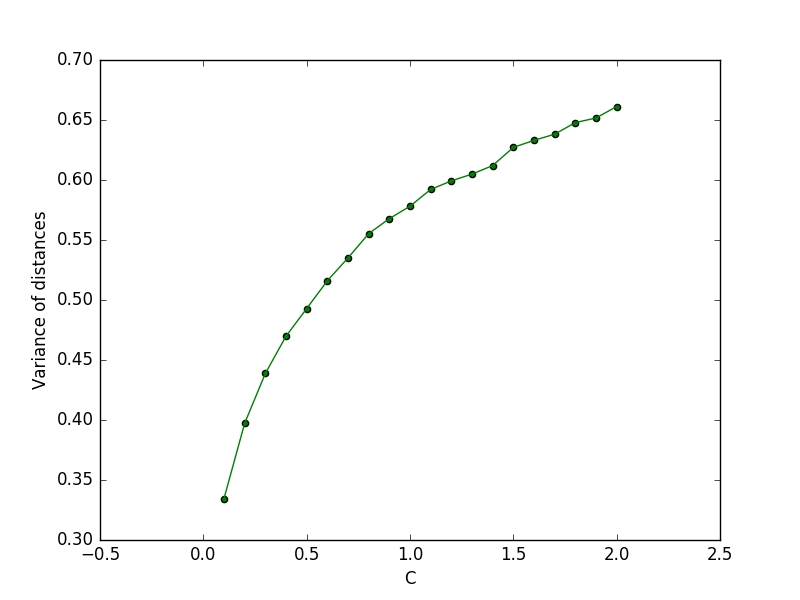
\includegraphics[width=1.5in]{abb/change_C_linear}}

\subfloat[]{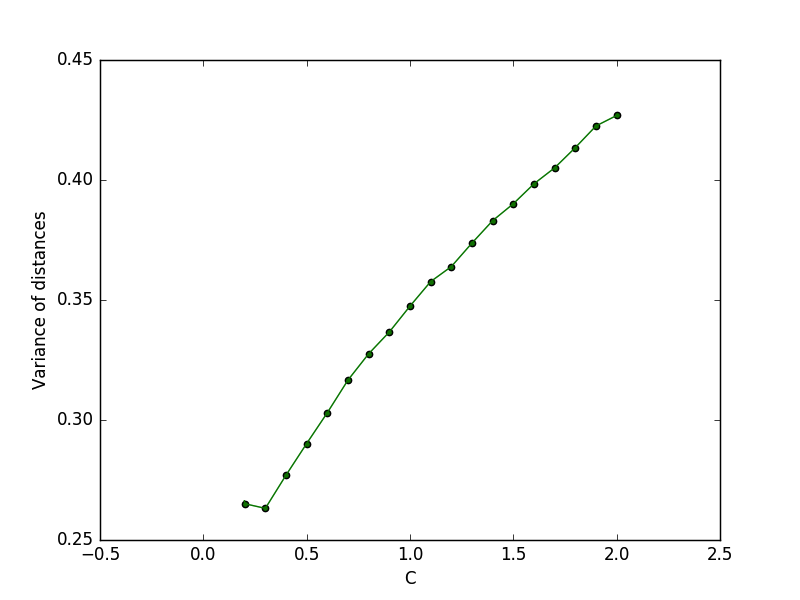
\includegraphics[width=1.5in]{abb/change_C_rbf}}
\caption{The results for chaning Balances linear Datasize 100 Repl 1000 Datasets 20}
\label{fig1}
\end{center}
\end{figure}


\subsection{Influence of the balance of the training dataset}


 Kernels are powerful! Kernels are powerful! Kernels are powerful! Kernels are powerful! Kernels are powerful! Kernels are powerful! Kernels are powerful! Kernels are powerful! Kernels are powerful! Kernels are powerful! Kernels are powerful! Kernels are powerful! Kernels are powerful! Kernels are powerful! Kernels are powerful! Kernels are powerful! Kernels are powerful! Kernels are powerful! Kernels are powerful! Kernels are powerful! Kernels are powerful! Kernels are powerful! Kernels are powerful! Kernels are powerful! Kernels are powerful! Kernels are powerful! Kernels are powerful! Kernels are powerful! Kernels are powerful! Kernels are powerful! Kernels are powerful! Kernels are powerful! Kernels are 

\begin{figure}[!htb]
\begin{center}
\subfloat[]{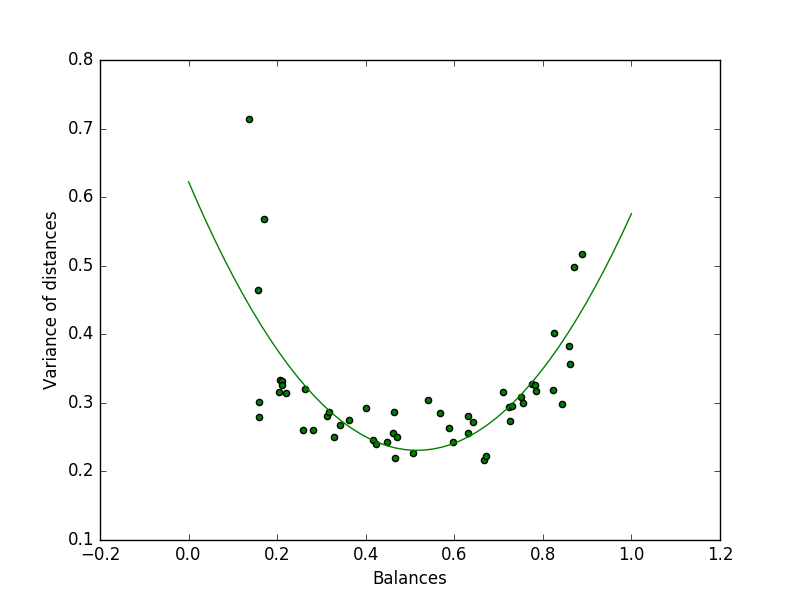
\includegraphics[width=1.5in]{abb/change_Balances_linear}}

\subfloat[]{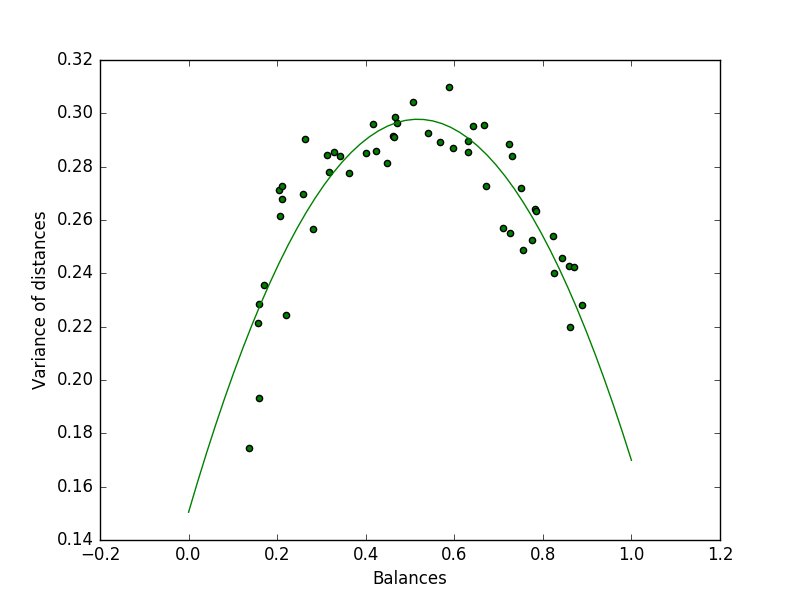
\includegraphics[width=1.5in]{abb/change_Balances_rbf}}
\caption{The results for chaning Balances linear Datasize 500 Repl 1000}
\label{fig1}
\end{center}
\end{figure}


\subsection{Influence of the svm attributes}
 Kernels are powerful! Kernels are powerful! Kernels are powerful! Kernels are powerful! Kernels are powerful! Kernels are powerful! Kernels are powerful! Kernels are powerful! Kernels are powerful! Kernels are powerful! Kernels are powerful! Kernels are powerful! Kernels are powerful! Kernels are powerful! Kernels are powerful! Kernels are powerful! Kernels are powerful! Kernels are powerful! Kernels are powerful! Kernels are powerful! Kernels are powerful! Kernels are powerful! Kernels are powerful! Kernels are powerful! Kernels are powerful! Kernels are powerful! Kernels are powerful! Kernels are powerful! Kernels are powerful! Kernels are powerful! Kernels are powerful! Kernels are powerful! Kernels are powerful! 

\begin{figure}[!htb]
\begin{center}
\subfloat[]{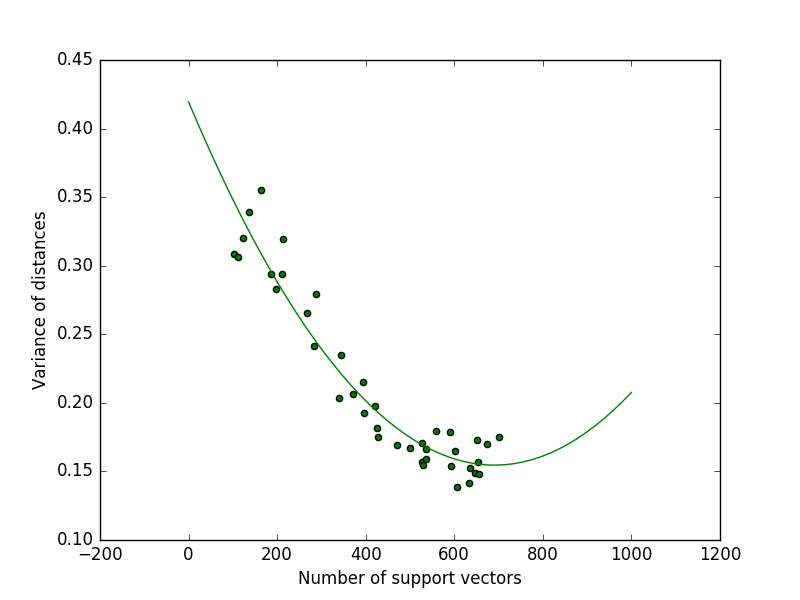
\includegraphics[width=1.5in]{abb/change_Support_Vectors_linear}}

\subfloat[]{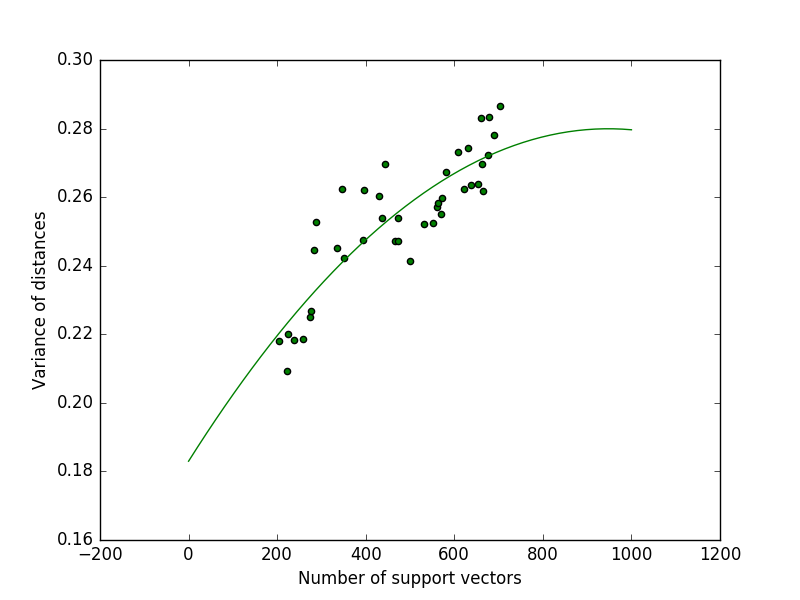
\includegraphics[width=1.5in]{abb/change_Support_Vectors_rbf}}
\caption{The results for chanching number of support vectors Datasize 1000 Repl 500}
\label{fig1}
\end{center}
\end{figure}


\section{Conclusion}
Nice to work with. I also works whit real datasets

Influence of different aspects on variance


C-Parameter: Positive but decreasing influence on variance. Balance of Data: Positive Quadratic influence for Linear and negative quadratic influence for Gaussian SVM. Both with extremum around 0.5 (perfect balance).
Number of support vectors: Positive influence for Gaussian and negative influence for linear SVMs

\section{Outlook}


Analyse influence of dimensionality on variances. Analyse Data simulated from more "exotic" distributions. Analyse influence of other tuning parameters e.g. "Gamma" of rbf-kernel, degree of polynomial kernel etc.




\footnotesize
\bibliographystyle{apalike}
\bibliography{sample}



\end{document}
